\section{Software performance}
Characterization of software performance is a complex problem, that
can be approached from different points of view. While software
developers are most concerned with understanding which parts of the
code need optimizing, for the computing infrastructure manager it is
mainly a question of measuring what is needed to run effectively the
experiment workloads. In this case, the application software is to be
considered, at a first approximation, as a ``black box'', and tools
like PrMon (which relies on the Linux kernel to extract CPU time,
memory, I/O and network metrics for a given process tree)~\cite{prmon}
or Trident (which gives access to detailed information on the CPU
utilization at the node level using hardware counters)~\cite{trident}
are extremely effective in producing metrics that can be used for
infrastructure planning, for benchmarking and for understanding
inefficiencies. As an example, Trident was used to quantify how much
the experiment workload are similar, or dissimilar, to a given
benchmark application, in how they use a CPU~\cite{bench}.

A set of reference workloads from each LHC experiment was analyzed
with PrMon, and the resulting values for the metrics are summarized in
table~\ref{table:prmon}. The metrics include: number of threads or
processes ($N_{thr/proc}$), CPU efficiency ($\epsilon_{CPU}$), time
per event ($T_{evt}$), memory per core ($M_c$), read rate per core
($R_c$) and write rate per core ($W_c$).

\begin{table}
\centering
\caption{Metrics measured by PrMon on a set of reference workloads with an Intel Xeon E5-2630. Values are approximate and may change with different versions of the experiment software}
\label{table:prmon}
\begin{tabular}{lrrrrrrrr}
\hline
job & $N_{thr/proc}$ & $\epsilon_{CPU}$ & $T_{evt}$ (s) & $M_{c}$ (GB) & $R_{c}$ (MB/s) & $W_{c}$ (MB/s) \\\hline
ALICE sim & 1 & 100\% & 10.9 & 0.96 & 0.08 & 0.17 \\
ATLAS G4 & 8 & 100\% & 270 & 0.44 & 0.015 & 0.009 \\
ATLAS digireco & 8 & 87\% & 56 & 1.1 & 0.3 & 0.24 \\
ATLAS deriv & 8 & 98\% & 0.7 & 1.2 & 0.7 & 0.07 \\
CMS gensim & 8 & 99\% & 21 & 0.2 & 0.05 & 0.04 \\
CMS digi & 8 & 78\% & 5.9 & 0.6 & 0.3 & 0.3 \\
CMS reco & 8 & 83\% & 9.8 & 0.45 & 0.3 & 0.2 \\
LHCb gensim & 1 & 100\% & 180 & 0.9 & 0.3 & 0.01 \\\hline
\end{tabular}
\end{table}
As the full PrMon output consists of time series for each metric, we
looked into ways to parametrize the time series using a minimal set of
parameters. A technique based on CPOP (Continuous piecewise linear
Pruned Optimal Partitioning)~\cite{cpop} is able to detect
changepoints and therefore reduce a time series to a very small number
of points (figure~\ref{fig:timeseries}). Another work looked into the
effect of varying limitations of system resources (memory, network
bandwidth and network latency) on the reference workloads, in
particular on their wall-clock time. It is planned to combine the two
analyses and study the results of the CPOP-based parametrization as
functions of the resource restrictions; this would allow to have a
very simple input to a future model of large scale workloads running
on a computing infrastructure, like a general purpose batch cluster or
an HPC resource.

\begin{figure}[t]
  \centering
  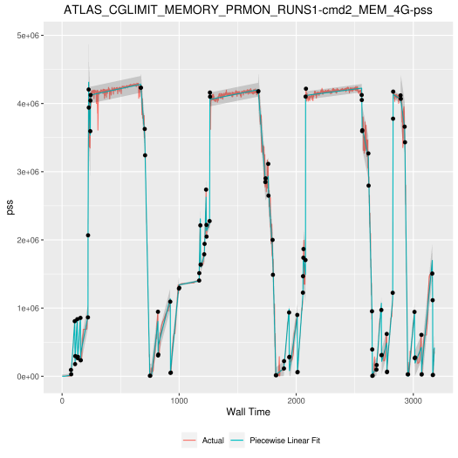
\includegraphics[height=6cm]{timeseries.png}
  \caption{Value of PSS vs. time for an ATLAS digi-reco job when the
    system memory is restricted to 4 GB}
  \label{fig:timeseries}
\end{figure}

Studies on the effect of compiler versions and optimizations were done
using Geant4 simulation, which showed that statically compiling
libraries may achieve a 10\% speedup with respect to dynamically
compiled libraries, and switching from gcc 4.8.5 to 8.2.0 resulted in
a 30\% speedup~\cite{marcon}. Consistent results were obtained for CMS
simulation~\cite{alejandro}.
